% L2a takeaway deck.
%
% THE DECK MIRRORS THE NOTEBOOK. The instructor shows
% CHEME-5660-L2a-Lecture-TreasurySecurities-Fall-2026.ipynb while students
% follow along and take notes on these slides. The deck therefore covers the
% same material in the same order, with frame titles matching notebook headings.
% Adding a section to the notebook means adding a slide here.
% See the content conventions in templates/vnslides.sty.
%
% Notebook outline, and where each part lands:
%
%   (deck only)                              -> title
%   Disclaimer and Risks          [last]     -> slide 2  (always near the front)
%   Learning Objectives           [cell 0]   -> Objectives for Today
%   Examples                                 -> Lectures and Examples
%   Concept Review                           -> transition frame + three review slides
%     Time Value of Money, Yields, ...       -> Review: Yields and Accumulation Factors
%     Abstract Assets and NPV                -> Review: Abstract Assets and NPV (+ NPV signs)
%   Treasury Bills                           -> bill types, cash flows, auction, and quotation slides
%     Valuing a T-Bill                       -> Valuing a T-Bill
%   Treasury Notes and Bonds                 -> cash flows, coupon/yield roles, and auction slides
%     Valuing Notes and Bonds                -> Valuing Notes and Bonds
%   Are Treasury securities risk-free?       -> Are Treasury Securities Risk-Free?
%     Case Studies: Sovereign Default Risk   -> Russia and Greece
%     Case Study: 2008 Financial Crisis      -> Case Study: 2008 Financial Crisis
%   Optional Advanced Material               -> Optional Advanced Material
%   Summary                                  -> Summary
%   Today?                                   -> closing transition frame
%
% Unlike L1b, this notebook DOES open with a concept-review section, so this deck
% uses \transitionframe as intended rather than as a 2024 holdover.
%
% Figures: L2a's figs/*.tex are standalone documents, not \input-able fragments
% the way L1b's abstract-asset-timeline.tex is, so the built PDFs are included
% directly. If those figures are ever refactored into fragments, switch to
% \resizebox{...}{!}{\input{...}} to match the L1b deck.
\documentclass[aspectratio=169,11pt]{beamer}
\usepackage{vnslides}

\title{{\vnheavy L2a}: Are Risk-Free Assets Really Risk-Free?}
\subtitle{CHEME 5660 Cornell University}
\author{Copyright Jeffrey Varner 2026. All Rights Reserved}

\begin{document}

% ---- title ---------------------------------------------------
\vntitlepage

% ---- disclaimer ----------------------------------------------
\begin{frame}{Disclaimer and Risks}
  \vspace{0.6em}
  \textbf{\ink{Training only.}} This content is for training and informational
  purposes only. The teaching team does not make, give, or endorse any offer or
  solicitation to buy or sell securities or derivative products, or provide
  investment or trading advice or strategy.

  \vspace{1.1em}
  \textbf{\ink{Risk.}} Trading involves risk and is generally not recommended for
  those with limited resources, experience, or a low risk tolerance. Past
  performance does not guarantee future success.

  \vspace{1.1em}
  \textbf{\ink{Responsibility.}} You are responsible for your investment decisions
  based on your financial circumstances, objectives, risk tolerance, and
  liquidity needs.
\end{frame}

% ---- objectives ----------------------------------------------
\begin{frame}{Objectives for Today}
  \vspace{0.4em}
  Today we introduce U.S. marketable Treasury securities, develop their cash-flow
  and pricing conventions, and ask what \hilite{risk-free} does and does not mean.

  \vspace{0.9em}
  {\large\textbf{\ink{Today's concepts}}}
  \vspace{0.4em}
  \begin{itemize}\setlength{\itemsep}{0.5em}
    \item \hilite{Describe Treasury securities}: distinguish regular bills, Cash
      Management Bills, notes, and bonds by their maturities and cash flows.
    \item \hilite{Value Treasury cash flows}: separate par from price and coupon
      rates from market yields, then use dated cash flows to calculate price.
    \item \hilite{Interpret the risk-free benchmark}: explain low default risk,
      changing market prices, and the flight to Treasuries during financial stress.
  \end{itemize}
  \vspace{-0.4em}

  \slidenote{Companion notebook:}{\href{https://github.com/varnerlab/CHEME-5660-CourseRepository-Fall-2026}{L2a lecture notebook}}
\end{frame}

% ---- examples ------------------------------------------------
\begin{frame}{Lectures and Examples}
  \vspace{0.5em}
  {\normalsize\textbf{\ink{Lecture:}} \dimmed{CHEME-5660-L2a-Lecture-TreasurySecurities-Fall-2026.ipynb}}

  \vspace{1.0em}
  The worked examples reconstruct reported auction prices from the Treasury's
  quotation conventions and actual auction data.

  \vspace{0.8em}
  {\normalsize\textbf{\ink{Example:}} \dimmed{CHEME-5660-L2a-TBills-Pricing-Fall-2026-WorkedExample.ipynb}}

  \vspace{0.2em}
  \dimmed{Zero-coupon bill auctions, 2023--2026.}

  \vspace{0.5em}
  {\normalsize\textbf{\ink{Example:}} \dimmed{CHEME-5660-L2a-NotesBonds-Pricing-Fall-2026-WorkedExample.ipynb}}

  \vspace{0.2em}
  \dimmed{Coupon note and bond auctions, 2022--2026.}

  \slidenote{Link:}{\href{https://github.com/varnerlab/CHEME-5660-CourseRepository-Fall-2026.git}{https://github.com/varnerlab/CHEME-5660-CourseRepository-Fall-2026.git}}
\end{frame}

% ---- concept review ------------------------------------------
\transitionframe{Quick review before we start: \hilite{the time value of money,
abstract assets, and net present value.}}

\begin{frame}{Review: Yields and Accumulation Factors}
  \hilite{Dated dollars have different units.} A dollar today and a dollar at a
  future date cannot be added until a stated rule expresses them at a common
  valuation date.

  \vspace{0.4em}
  Let $P$ be an amount held today, let $y$ be a quoted \hilite{nominal annual
  yield}, and let $n$ be the number of compounding intervals per year. At period
  index $j$, the equivalent future amount is given by:
  \[
    F_j=\underbrace{\left(1+y/n\right)^{j}}_{\mathcal D_{j,0}(y;n)}\,P .
  \]

  $\mathcal D_{j,0}(y;n)$ converts time-0 dollars into period-$j$ dollars and its
  inverse converts them back. The continuously compounded equivalent is
  $g_y:=n\log(1+y/n)$, so $\mathcal D_{T,0}(y;n)=(1+y/n)^{nT}=e^{g_yT}$ over $T$
  years.

  \slidenote{Careful:}{$g$ is a growth rate and $r=(\Delta t)\,g$ its log return. Convert a quoted $y$ before comparing.}
\end{frame}

\begin{frame}{Review: Abstract Assets and Net Present Value}
  \vspace{0.3em}
  \hilite{Abstract assets} describe financial value as dated signed cash flows.
  Because dated dollars have different units, each cash flow must be converted to
  a common valuation date before the values are added.

  \vspace{0.5em}
  Let $N$ be the final cash-flow index and let $\bar c_j$ be the \hilite{signed
  net cash flow} at index $j$. Under a constant nominal yield $y$, the time-0 net
  present value is given by:
  \[
    \operatorname{NPV}_{0}(y)=\sum_{j=0}^{N}\mathcal D_{j,0}^{-1}(y;n)\,\bar c_j .
  \]

  \vspace{0.3em}
  Every term in the sum is measured in time-0 dollars.

  \slidenote{Today:}{set $\operatorname{NPV}_0=0$ and solve for the price. That is what pricing a Treasury security means.}
\end{frame}

\begin{frame}{The NPV Sign Is a Valuation Test}
  Once every cash flow is expressed in today's dollars, NPV asks whether the
  present value received is greater than, less than, or equal to the amount paid.

  \vspace{0.5em}
  \begin{itemize}\setlength{\itemsep}{0.55em}
    \item \textbf{\ink{Positive NPV:}} present value received $>$ amount paid;
      the asset clears the chosen discount-rate benchmark.
    \item \textbf{\ink{Negative NPV:}} present value received $<$ amount paid;
      the asset does not clear that benchmark.
    \item \textbf{\ink{Zero NPV:}} present value received $=$ amount paid; this is
      the pricing condition used for Treasury securities.
  \end{itemize}

  \vspace{0.3em}
  \hilite{The sign is conditional on the discount model and assumed cash flows; it
  is not a promise about what will happen.}
\end{frame}

% ---- T-bills -------------------------------------------------
\begin{frame}{Treasury Bills}
  A U.S. Treasury bill is a short-term \hilite{zero-coupon debt security}: the
  investor receives no periodic coupon and is paid the par amount at maturity.

  \vspace{0.6em}
  \begin{itemize}\setlength{\itemsep}{0.55em}
    \item \textbf{\ink{Regular Treasury bills}} have standardized 4-, 6-, 8-,
      13-, 17-, 26-, or 52-week terms and follow a recurring auction schedule.
      Investors may use TreasuryDirect or a bank, broker, or dealer.
    \item \textbf{\ink{Cash Management Bills (CMBs)}} have variable terms from a
      few days to one year and are auctioned only when Treasury needs them. They
      must be purchased through a bank, broker, or dealer.
  \end{itemize}

  \vspace{0.2em}
  Their scheduling and access differ, but their \hilite{cash-flow and valuation
  mechanics are the same}.

  \slidenote{Sources:}{\href{https://www.treasurydirect.gov/marketable-securities/treasury-bills/}{Treasury bills}; \href{https://www.treasurydirect.gov/marketable-securities/cash-management-bills/}{Cash Management Bills}.}
\end{frame}

\begin{frame}{Treasury Bill Cash Flows}
  \vspace{0.2em}
  \begin{center}
    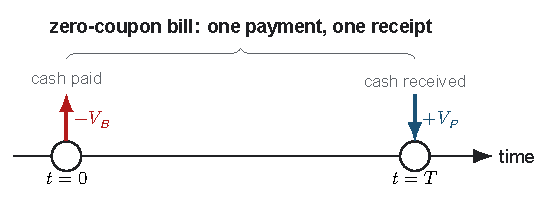
\includegraphics[width=\textwidth,height=0.66\textheight,keepaspectratio]{../figs/Fig-L2a-TBill-CashFlows.pdf}
  \end{center}
\end{frame}

\begin{frame}{Par Amount, Purchase Price, and Discount}
  A bill has two investor cash flows: the purchase price $-V_B$ today and the
  par payment $+V_P$ at maturity.

  \vspace{0.6em}
  \begin{itemize}\setlength{\itemsep}{0.55em}
    \item \textbf{\ink{Par amount $V_P$:}} the fixed amount Treasury promises to
      pay at maturity.
    \item \textbf{\ink{Purchase price $V_B$:}} the cash paid to acquire the bill;
      it is normally below par at auction.
    \item \textbf{\ink{Dollar discount $V_P-V_B$:}} the interest earned when a
      below-par bill is held to maturity.
  \end{itemize}

  \vspace{0.4em}
  \hilite{Par determines the maturity payment; price determines the amount
  invested.} The dollar discount is not a rate until a horizon and quotation
  convention are specified.
\end{frame}

\begin{frame}{Two Ways to Bid at a T-Bill Auction}
  Treasury uses a \hilite{single-price auction}: every bidder who receives bills
  pays the same auction price.

  \vspace{0.6em}
  \begin{itemize}\setlength{\itemsep}{0.7em}
    \item \textbf{\ink{Noncompetitive bid:}} Most individual investors request a
      par amount and accept the auction-determined rate. Within the auction
      limit, the requested par amount is guaranteed; TreasuryDirect offers only
      this bid type.
    \item \textbf{\ink{Competitive bid:}} Institutional and other experienced
      investors request a par amount and state the minimum bank discount rate
      they will accept. They gain control over the minimum return but risk a
      partial award or no award. These bids go through a bank, broker, or dealer.
  \end{itemize}

  \slidenote{Source:}{\href{https://www.treasurydirect.gov/auctions/how-auctions-work/}{TreasuryDirect: How Auctions Work}.}
\end{frame}

\begin{frame}{A Competitive Bid Controls Allocation, Not Price}
  Let $d^*$ be the auction \hilite{cutoff rate}: the highest competitive bank
  discount rate to receive an award. A bidder requesting par amount $V_P$ gets:
  \[
    \begin{array}{ccl}
      d<d^* &\Longrightarrow& 100\%\text{ of requested par},\\[0.25em]
      d=d^* &\Longrightarrow& \text{possibly a prorated share of requested par},\\[0.25em]
      d>d^* &\Longrightarrow& \text{no award}.
    \end{array}
  \]

  If a bidder requests $10{,}000~\mathrm{USD}$ of par, a full award is
  $10{,}000~\mathrm{USD}$ of par; a $60\%$ proration is $6{,}000~\mathrm{USD}$ of
  par. These are \hilite{award amounts, not cash prices}.

  \vspace{0.4em}
  Treasury computes one price from $d^*$, and every awarded bidder pays that
  price per $100~\mathrm{USD}$ of par.

  \slidenote{Source:}{\href{https://www.treasurydirect.gov/help-center/faqs/additional-auction-related-faqs/}{TreasuryDirect auction allocation and proration}.}
\end{frame}

\begin{frame}{From Bank Discount Rate to Auction Price}
  If a bill has $D$ days to maturity, its bank discount rate $d$ implies:
  \[
    \boxed{V_B=V_P\left(1-d\frac{D}{360}\right)} .
  \]

  \vspace{0.4em}
  Treasury reports the price per $100~\mathrm{USD}$ of par, so set
  $V_P=100~\mathrm{USD}$.

  \vspace{0.5em}
  \begin{itemize}\setlength{\itemsep}{0.45em}
    \item A price of $99.72~\mathrm{USD}$ means the investor pays
      $99.72~\mathrm{USD}$ today for $100~\mathrm{USD}$ at maturity.
    \item If held to maturity, the dollar interest is
      $100-99.72=0.28~\mathrm{USD}$ per $100~\mathrm{USD}$ of par.
  \end{itemize}

  \hilite{The bank discount convention uses par value and a 360-day year.}

  \slidenote{Source:}{\href{https://www.treasurydirect.gov/marketable-securities/understanding-pricing/}{TreasuryDirect: Understanding Pricing}.}
\end{frame}

\begin{frame}{Valuing a T-Bill}
  Let $y$ be a nominal annual yield used for valuation, let $n$ be its compounding
  frequency, and define $g_y=n\log(1+y/n)$. Setting NPV to zero gives:
  \[
    V_B=\mathcal D_{T,0}^{-1}(y;n)\,V_P=\left(1+\frac{y}{n}\right)^{-nT}V_P=e^{-g_yT}V_P .
  \]

  The price-implied annualized log yield and holding-period log return are:
  \[
    g_B=\frac{1}{T}\log\left(\frac{V_P}{V_B}\right),
    \qquad r_B=T\,g_B .
  \]

  When $V_B$ is the model price, $g_B=g_y$. When $V_B$ is an observed market
  price, $g_B$ is implied by that price and may differ from the model input.

  \vspace{0.4em}
  \hilite{Zero NPV does not mean zero return or zero risk.} It means the price
  reflects the return required by the market under the stated model.
\end{frame}

\begin{frame}{A \$100 T-Bill: Price, Gain, and Return}
  A $100~\mathrm{USD}$ bill matures in six months. Use nominal annual yield
  $y=5\%$ with semiannual compounding, so $n=2$ and $T=0.5$ year.
  \begin{align*}
    V_B &=100(1.025)^{-1}=97.56098\approx 97.56~\mathrm{USD},\\
    V_P-V_B &\approx 2.44~\mathrm{USD},\\
    g_B &=2\log(1.025)\approx 4.9385\%\text{/year},\\
    r_B &=\log(1.025)\approx 2.4693\%\text{ over six months}.
  \end{align*}

  \hilite{Annualized growth and holding-period return are different quantities.}

  \vspace{0.45em}
  Treasury bank-discount and investment-yield quotations are not automatically
  $y$ or $g_y$; match day-count and compounding conventions before comparing.

  \slidenote{Formulas:}{\href{https://www.treasurydirect.gov/files/laws-and-regulations/auction-regulations-uoc/auct-reg-gsr-356122303.pdf}{official Treasury auction formulas}.}
\end{frame}

% ---- notes and bonds -----------------------------------------
\begin{frame}{Treasury Notes and Bonds}
  \vspace{0.2em}
  Treasury notes and bonds are fixed-rate coupon securities that pay interest
  every six months and repay par at maturity.

  \vspace{0.45em}
  \begin{itemize}\setlength{\itemsep}{0.35em}
    \item \textbf{\ink{Notes:}} original terms of 2, 3, 5, 7, or 10 years.
    \item \textbf{\ink{Bonds:}} original terms of 20 or 30 years.
  \end{itemize}

  \vspace{0.5em}
  At original issue, semiannual payments imply $n=2$ and $N=nT$ coupon dates. In
  a reopening or secondary-market trade, $N$ means the number of remaining
  coupons. If $c$ is the annual coupon rate, each coupon is $C=(c/n)V_P$:
  \[
    \bar c_0=-V_B,
    \qquad
    \bar c_j=C \;\; (j=1,\ldots,N-1),
    \qquad
    \bar c_N=C+V_P .
  \]

  \slidenote{Sources:}{\href{https://www.treasurydirect.gov/marketable-securities/treasury-notes/}{Treasury notes}; \href{https://www.treasurydirect.gov/marketable-securities/treasury-bonds/}{Treasury bonds}.}
\end{frame}

\begin{frame}{Note and Bond Cash Flows}
  \vspace{0.2em}
  \begin{center}
    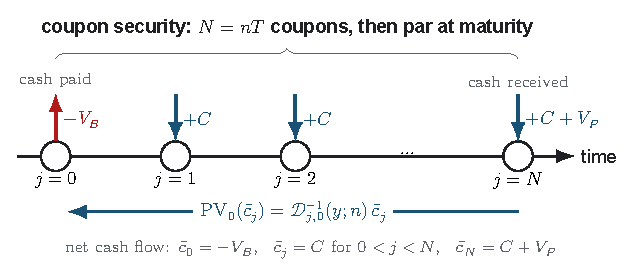
\includegraphics[width=\textwidth,height=0.66\textheight,keepaspectratio]{../figs/Fig-L2a-NoteBond-CashFlows.pdf}
  \end{center}
\end{frame}

\begin{frame}{Coupon Rate and Market Yield Do Different Jobs}
  The coupon rate fixes the promised cash flows; the market yield determines
  what those cash flows are worth today.

  \vspace{0.6em}
  \begin{itemize}\setlength{\itemsep}{0.55em}
    \item \textbf{\ink{Par amount $V_P$:}} fixed principal repaid at maturity.
    \item \textbf{\ink{Coupon rate $c$:}} fixed after issue and determines each
      semiannual payment, $C=(c/2)V_P$.
    \item \textbf{\ink{Market yield $y$:}} the return required for the remaining
      cash flows; it changes with market conditions.
    \item \textbf{\ink{Price $V_B$:}} the present value of the remaining coupons
      and par payment discounted at $y$, so it changes when $y$ changes.
  \end{itemize}

  \vspace{0.3em}
  \hilite{At an original-issue auction, competitive bidders specify yields, not
  coupon rates.}
\end{frame}

\begin{frame}{The Auction Yield Sets the Coupon and Price}
  The highest competitive yield to receive an award is the \hilite{high yield}
  $y^*$. It determines the common auction price; bids below $y^*$ receive the
  full requested par amount, bids at $y^*$ may be prorated, and bids above it
  receive nothing.

  \vspace{0.6em}
  After the auction, Treasury chooses a coupon rate in $0.125$-percentage-point
  increments that prices the security closest to, but not above, par.

  \vspace{0.7em}
  \textbf{\ink{August 12, 2026 example}}
  \begin{itemize}\setlength{\itemsep}{0.35em}
    \item High yield: $y^*=4.683\%$.
    \item Coupon rate selected: $c=4.625\%$.
    \item Auction price: $99.5407~\mathrm{USD}$ per $100~\mathrm{USD}$ of par.
  \end{itemize}

  \slidenote{Sources:}{\href{https://www.treasurydirect.gov/marketable-securities/understanding-pricing/}{TreasuryDirect pricing}; \href{https://www.ecfr.gov/current/title-31/subtitle-B/chapter-II/subchapter-A/part-356/section-356.20}{31 CFR 356.20}.}
\end{frame}

\begin{frame}{Valuing Notes and Bonds}
  Assume valuation occurs on a coupon date, with $N$ complete coupon periods
  remaining. Let $y$ be the nominal annual YTM compounded semiannually. Setting
  NPV to zero and solving for price gives:
  \begin{align*}
    0 &= \underbrace{-V_B}_{\text{\footnotesize cost}}
       + \underbrace{\mathcal D_{N,0}^{-1}(y;n)V_P}_{\text{\footnotesize par payment}}
       + \underbrace{C\sum_{j=1}^{N}\mathcal D_{j,0}^{-1}(y;n)}_{\text{\footnotesize coupon payments}}\\[0.3em]
    V_B &= \mathcal D_{N,0}^{-1}(y;n)V_P+C\sum_{j=1}^{N}\mathcal D_{j,0}^{-1}(y;n),
    \qquad \mathcal D_{j,0}^{-1}(y;n)=\left(1+\frac{y}{n}\right)^{-j}.
  \end{align*}

  \vspace{0.2em}
  This YTM convention discounts every payment at the same rate. A term-structure
  valuation instead uses a maturity-specific spot rate for each cash flow.
\end{frame}

% ---- risk ----------------------------------------------------
\begin{frame}{Are Treasury Securities Risk-Free?}
  \vspace{0.3em}
  U.S. Treasury securities are commonly treated as \hilite{low-default-risk
  nominal-dollar benchmarks}. That does not make every government security---or
  every debt instrument issued in the United States---risk-free.

  \vspace{0.65em}
  \begin{itemize}\setlength{\itemsep}{0.55em}
    \item \textbf{\ink{Default risk:}} the borrower may miss, suspend, or
      restructure a promised payment. The central question is: \emph{who promised
      the payment, and under what terms?}
    \item \textbf{\ink{Interest-rate risk:}} when market yields change, Treasury
      prices change. Selling before maturity may realize a gain or loss even when
      every promised payment is ultimately made.
  \end{itemize}

  \vspace{0.4em}
  During financial stress, investors often move toward Treasuries in a
  \hilite{flight to quality}; the label is relative, not absolute.
\end{frame}

\begin{frame}{Sovereign Debt Can Default or Be Restructured}
  Government debt is not inherently free of default risk. Two recent sovereign
  examples changed the timing or amount of promised payments:

  \vspace{0.6em}
  \begin{itemize}\setlength{\itemsep}{0.65em}
    \item \textbf{\ink{Russia, 1998:}} On August 17, Russia announced a de facto
      default and restructuring of ruble-denominated government bills and bonds.
      Creditors suffered losses, and the event amplified an international
      financial and liquidity crisis.
    \item \textbf{\ink{Greece, 2012:}} About $97\%$ of the privately held bonds
      covered by the exchange participated; investors accepted a $53.5\%$
      reduction in face value.
  \end{itemize}

  \vspace{0.35em}
  Both the probability of default and the amount recovered after default affect
  a security's value.

  \slidenote{Sources:}{\href{https://www.imf.org/en/news/articles/2015/09/14/01/49/pr9935}{IMF: Russia}; \href{https://www.esm.europa.eu/content/what-was-private-sector-debt-restructuring-march-2012}{ESM: Greece}.}
\end{frame}

\begin{frame}{Mortgage Defaults and the 2008 Financial Crisis}
  The housing collapse shows why the identity of the borrower and the structure
  of the promised payments matter.

  \vspace{0.55em}
  \begin{itemize}\setlength{\itemsep}{0.45em}
    \item Falling house prices drove mortgage delinquencies and defaults.
    \item Losses spread through widely held mortgage-backed securities.
    \item Leverage and short-term funding amplified the damage and uncertainty
      about counterparties.
    \item Investors fled toward U.S. Treasuries in a \hilite{flight to quality}.
  \end{itemize}

  \vspace{0.35em}
  Mortgage-backed securities and Treasuries were both dollar-denominated debt but
  had different borrowers, cash flows, and default risks. The Financial Crisis
  Inquiry Commission concluded that the crisis was avoidable and warnings were
  ignored.

  \slidenote{Explore:}{\href{https://www.youtube.com/watch?v=GPOv72Awo68}{short overview}; \href{https://www.govinfo.gov/content/pkg/GPO-FCIC/pdf/GPO-FCIC.pdf}{Financial Crisis Inquiry Commission Report}.}
\end{frame}

% ---- optional advanced material ------------------------------
\begin{frame}{Optional Advanced Material}
  \vspace{0.2em}
  {\normalsize\textbf{\ink{Advanced 1:}} \dimmed{advanced/default-risk/}\par
  \dimmed{CHEME-5660-L2a-Advanced-Bernoulli-DefaultRisk-Fall-2026.ipynb}}

  \vspace{0.5em}
  Optional; not a prerequisite for L2b. The example represents principal and
  coupon payments with Bernoulli survival indicators, adds recovery following
  default, and verifies the analytical expected-value price with a Monte Carlo
  simulation.
  \slidenote{Notebooks:}{\href{https://github.com/varnerlab/CHEME-5660-CourseRepository-Fall-2026/tree/main/lectures/week-2/L2a/advanced}{lectures/week-2/L2a/advanced}, also linked from the lecture notebook.}
\end{frame}

% ---- summary -------------------------------------------------
\begin{frame}{Summary}
  This lecture introduced the cash-flow structures, valuation, and risks of U.S.
  Treasury securities.

  \vspace{0.45em}
  {\large\textbf{\ink{Key takeaways}}}
  \vspace{0.2em}
  \begin{itemize}\setlength{\itemsep}{0.35em}
    \item \textbf{\ink{Cash flows determine value.}} A bill's par amount is its
      maturity payment, not necessarily its purchase price. Notes and bonds pay
      coupons and return par. Price puts every cash flow at one valuation date.
    \item \textbf{\ink{Coupon rates and yields do different jobs.}} The coupon
      rate fixes promised payments; the market yield discounts them and determines
      price. Quotation, day-count, compounding, and accrued-interest conventions
      must match before prices or rates are compared.
    \item \textbf{\ink{Risk-free is a relative term.}} Treasuries have low
      nominal default risk and often attract investors during stress, but their
      prices can still fall when yields rise.
  \end{itemize}

  \vspace{0.5em}
  Treasury securities connect dated cash flows, discounting, and market risk.
\end{frame}

% ---- closing -------------------------------------------------
\transitionframe{That's a wrap. \hilite{What are some of the interesting things
we discussed today?}}

\end{document}
